\documentclass[a4paper,12pt,twoside]{article}
\usepackage[left=1in,right=1in,top=1in,bottom=1in]{geometry}

\input{../styles/preamble.tex}
\input{../styles/Chinese_math_style.tex}
\input{../styles/math_style.tex}

\newcommand{\redtext}[1]{{\color{red} #1}}
\newcommand{\bluetext}[1]{{\color{blue} #1}}

\fancypagestyle{firstpage}{
  \fancyhf{}
  \fancyhead[R]{\small《高中數學實驗教材》第 1 冊}
  \fancyhead[L]{\small 第 2 章\quad 符號用法、基本數學語句及集合的概念}
  \fancyfoot[C]{\thepage}
}

\pagestyle{fancy}
\renewcommand{\headrulewidth}{0.5pt}
\renewcommand{\footrulewidth}{0pt}
\fancyhead{}
\fancyhead[LE]{\small 《高中數學實驗教材》第一冊}
\fancyhead[RO]{\small 第二章\quad 符號用法、基本數學語句及集合的概念}
\fancyfoot[C]{\thepage}

\title{\LARGE\textbf{《高中數學實驗教材》第一冊}\\[0.5em] \Large\textbf{第二章\quad 符號用法、基本數學語句及集合的概念}}
\author{\textbf{高中數學實驗教材編輯小組}\quad 編著}
\date{民國六十二年（1973）修訂版}

\begin{document}

\maketitle
\thispagestyle{firstpage}

% ==========================================
% 第二章 掃描檔勘誤、文字校訂與疑難處說明（依規則 6 整理於目錄之前）
% ==========================================
\section*{【說明】第二章 掃描檔勘誤、疑難處與文義校訂表}
\addcontentsline{toc}{section}{【說明】第二章 掃描檔勘誤、疑難處與文義校訂表}
\label{sec:ch2_errata_notes}

本章依據 1973 年版《高中數學實驗教材 第一冊》（高一上）第二章「符號用法、基本數學語句及集合的概念」33 頁掃描原件（第 13 頁至第 45 頁）完整轉錄為 \LaTeX{} 格式。依作業規範將掃描檔中出現之排印訛誤、數據手民之誤、符號缺漏、字模損毀及文義疑難處詳細考證彙整於下表：

\begin{table}[H]
\centering
\small
\renewcommand{\arraystretch}{1.35}
\begin{tabularx}{\textwidth}{|p{3.2cm}|p{3.8cm}|X|}
\hline
\textbf{章節位置} & \textbf{掃描檔原始現象 / 誤植} & \textbf{考證說明與校訂處理} \\ \hline

\hyperref[subsec:2-3-a]{2.3 甲 康托生卒年} & 
「康托(George Cantor, 11845-1918)所著」 & 
出生年份「11845」顯為多排一個「1」之鉛字訛誤，正文校訂為「1845--1918」。 \\ \hline

\hyperref[subsec:2-3-f]{2.3 己 例 1 新生社團} & 
題目文字印為「357人三樣都參加」 & 
題目敘述中之「357人」與下文圖形、算式「$35$ 人」及總人數「$762$ 人」矛盾，顯為鉛字排印誤植「7」字。依算式邏輯校訂為「35 人三樣都參加」。 \\ \hline

\hyperref[sec:ex2-3]{習題 2-3 頁首書眉} & 
書眉印為「第二章 符號用法,基本數學語句及集各的概念」 & 
「集各」為「集合」之排印訛字，正文與書眉校補為「集合」。 \\ \hline

\hyperref[sec:ex2-4]{習題 2-4 第 3(i) 題} & 
「$\triangle ABC, \angle B=90^\circ$ 的充分必要條件是 $AC^2+BC^2=AC^2$」 & 
算式中重複出現 $AC^2$，依畢氏定理斜邊應為 $AC$、兩股為 $AB, BC$，校正為 $AB^2+BC^2=AC^2$。 \\ \hline

\hyperref[subsec:2-4-d]{2.4 丁 補集符號} & 
原書同時使用「$\sim A$」與波浪號「$\sim$」表示補集與否定 & 
維持原書「$\sim A$」及「$\sim \alpha$」之特殊符號風格，精確反映 1970 年代實驗教材引進現代邏輯與集合論時之原始語法。 \\ \hline

\hyperref[sec:ch2-appendix]{附錄：羅馬乘法} & 
羅馬數字繁複分配律乘法演算 & 
依原書第 45 頁附錄完整收錄並以對齊數學環境重現，展示印度--阿拉伯記數系統相對於羅馬數字之優越性。 \\ \hline

\end{tabularx}
\end{table}

\clearpage
\tableofcontents
\newpage

% =========================================================================
% 《高中數學實驗教材》第一冊（高一上）
% 第二章 符號用法、基本數學語句及集合的概念
% =========================================================================

\section{符號用法、基本數學語句及集合的概念}\label{sec:ch2}

「符號」是數學中用以表達意思、討論問題的「文字」，「集合」的概念是我們在日常生活中常用的，在數學裏只是把它加以明確的解釋，然後廣泛地用來討論種種數學問題。

\subsection{符號在數學中的用法}\label{sec:2-1}

自遠古人類結繩記事以來，「符號」一直被我們廣泛地用來記事、指標、表達意見和思想等等，而各民族的「文字」也就是由「約定俗成」所產生的一套有系統的符號。通常一個單字就是一個特定的符號，約定用來表示某一事物、動作或觀念等等；而一個句子就是把一些單字依文法適當地串連起來，用以表達思想、交換意見。在數學裏，我們將更加徹底而有效地利用符號。符號在數學中的用法和我們日常文字的用法大同小異，現在比較其異同如下：

\subsubsection*{甲、符號意義的約定與賦予}\label{subsec:2-1-a}

在日常文字中，一個單字的意義是由約定俗成而定的，它的意義在字典裏有詳盡的記載。在數學中，只有很少幾個基本常用的符號如「$+$」、「$-$」、「$0$」、「$1$」……等，它們的意義也是約定俗成而定的，多為全世界通用。但是在數學中大部分的符號，它們的意義是我們對於某一章、某一節，或某一問題所臨時賦予的。

譬如當我們用代數方程式去解某一雞兔問題時，我們開宗明義地「令 $x$ 為雞的個數」，那麼，在該問題的討論過程中，「$x$」就永遠表示「雞數」；反之，假如一開始我們「令 $x$ 為兔的個數」，則在該問題的討論中，「$x$」就永遠表示「兔數」。

所以同學們在讀數學書時，一定要切實弄清楚在這一章、這一節中每一符號的意義，切不可把不同章、節中的「同形狀符號」混為一談，因為同一符號在不同的地方是可以被賦予不同的意義的！只要同學們從今天起，養成習慣在每一章、每一節的開始，切切實實地弄清楚其中所用的符號的定義，那麼數學中這種符號活用的辦法，是又方便又簡捷的。

\subsubsection*{乙、符號意義的明確性}\label{subsec:2-1-b}

在日常文字中，一個單字常常有好幾個不同的意義，當它被用在某一個句子中，往往要看上下文才能決定採用哪一個意義。有時候，可能好幾個意義都可以講得通，譬如所謂「雙關語」就是一例。

但是數學是一門嚴格的科學，所以在某一章節或某一問題的討論過程中，所用的每一符號的意義必須是明確的。

\subsection{數學符號運用的要領}\label{sec:2-2}

數學裏對於符號的選取在理論上是相當自由的，我們只要在符號引入時加以明確的定義就可以。但是在實際運用時，符號的選取是有些講究的，一般說來，我們應該注意下列幾點：

\subsubsection*{甲、易於辨識與書寫簡便}\label{subsec:2-2-a}

所用的符號應儘可能容易辨識，而且書寫簡便。再者，一些常常同時出現的幾種符號，最好不要很相似，以免混淆。

\begin{example}\label{ex:2-2-1}
在算術中，「小數點」是一個常用的符號，那時我們還沒有引進「未知數」，並不用「$x$」這個字母，所以在算術中我們用「$\times$」表示「乘號」而不用「$\cdot$」去表示「乘號」。

到了初中學代數時，「$x$」這個字母是常常出現的，但是「小數點」卻較少用到（我們很容易地可以用分數去表示小數），所以在代數中我們用「$\cdot$」表示「乘號」而不用「$\times$」去表示「乘號」，這就是避免太相似的符號常常同時出現的一個實例。
\end{example}

\subsubsection*{乙、明確為第一要義，次求簡便與系統化}\label{subsec:2-2-b}

在數學符號的運用上，「明確」是一個絕對不可或缺的要素！在具備「明確」這一要素後，我們才再去求簡便、求系統化。

\begin{example}\label{ex:2-2-2}
為了說明上述要領，我們且以「自然數」為例，和同學們比較一下自然數的幾種符號間的優劣。

\begin{enumerate}[(1)]
  \item 「自然數」的一種最原始的符號也許是：
  \begin{equation*}
    |, \quad ||, \quad |||, \quad ||||, \quad |||||, \quad \dots
  \end{equation*}
  上面這一套符號雖然夠明確，但是稍大一點的數目如「三百六十五」，寫起來就不勝其繁了。

  \item 古代羅馬人將上述符號加以改進，他們用符號：
  \begin{itemize}
    \item 用「$\mathrm{V}$」去代替「$|||||$」，
    \item 用「$\mathrm{X}$」去代替「$\mathrm{VV}$」，
    \item 用「$\mathrm{L}$」去代替「$\mathrm{XXXXX}$」，
    \item 用「$\mathrm{C}$」表示「百」，
    \item 用「$\mathrm{D}$」表示「五百」，
    \item 用「$\mathrm{M}$」表示「千」。
  \end{itemize}
  所以古羅馬的「數字」如下：
  \begin{equation*}
    \mathrm{I, II, III, IIII, V, VI, VII, VIII, VIIII, X, XI, \dots, CCCLXV, MLXI, \dots}
  \end{equation*}
  （即 $1, 2, 3, 4, 5, 6, 7, 8, 9, 10, 11, \dots, 365, \dots, 1061, \dots$）。

  可是後來羅馬人嫌「$\mathrm{IIII}$」、「$\mathrm{VIIII}$」、「$\mathrm{XXXX}$」等寫起來太繁，於是大家約定：「當小單位於大單位之前時表示減」，這樣：
  \begin{itemize}
    \item 「$\mathrm{IIII}$」就可以簡寫為「$\mathrm{IV}$」，
    \item 「$\mathrm{VIIII}$」就可以簡寫為「$\mathrm{IX}$」，
    \item 「$\mathrm{XXXX}$」就可以簡寫為「$\mathrm{XL}$」，「$\mathrm{LXXXX}$」就可以簡寫為「$\mathrm{XC}$」，……以此類推。
  \end{itemize}
  同學們可以看出來，羅馬人的記數符號依然是很原始的，他們只是多了幾個縮寫「$\mathrm{V, X, L, C, D, M}$」可以把較大的數寫得簡短些。在羅馬時代，由於記數符號的不理想，兩個較大的數相乘，就成了個困難的計算問題（見\hyperref[sec:ch2-appendix]{附錄}）。

  \item 現代通用的記數符號，源自印度、阿拉伯，其原理在於有效地利用指數定則、分配律等數的運算法則。我們以 $10, 10^2, 10^3, \dots$ 等 $10$ 的冪方作為「輔助單位」，可以把任何自然數用 $0, 1, 2, 3, 4, 5, 6, 7, 8, 9$ 這十個符號簡潔而有系統地加以表示，譬如：
  \begin{itemize}
    \item 用「$365$」表示「三百六十五」$= 3 \times 10^2 + 6 \times 10 + 5$；
    \item 用「$90503$」表示「九萬五百零三」$= 9 \times 10^4 + 5 \times 10^2 + 3$；
    \item 用「$4007$」表示「四千零七」$= 4 \times 10^3 + 7$。
  \end{itemize}
  上述記數的符號體系，不但簡潔明確，而且用來計算加、減、乘、除等基本運算時，又十分便捷。譬如讓我們來算一算一年有幾小時？

  若不是閏年，則一年有 $365$ 天，一天有 $24$ 小時，所以我們要計算 $365 \times 24$ 如下：
  \begin{align*}
    365 \times 24 &= (3 \times 10^2 + 6 \times 10 + 5) \times (2 \times 10 + 4) && \text{〔記數符號的定義〕} \\
    &= (3 \times 10^2 + 6 \times 10 + 5) \times (2 \times 10) + (3 \times 10^2 + 6 \times 10 + 5) \times 4 && \text{〔分配律〕} \\
    &= \{(3 \times 2) \times 10^2 \times 10 + (6 \times 2) \times 10 \times 10 + (5 \times 2) \times 10\} \\
    &\quad + \{3 \times 4 \times 10^2 + 6 \times 4 \times 10 + 5 \times 4\} && \text{〔分配律〕} \\
    &= \{6 \times 10^3 + 12 \times 10^2 + 10 \times 10\} + \{12 \times 10^2 + 24 \times 10 + 20\} && \text{〔九九表及指數定則 $10^a \cdot 10^b = 10^{a+b}$〕} \\
    &= 6 \times 10^3 + (10^3 + 2 \times 10^2) + 10^2 + (10^3 + 2 \times 10^2) \\
    &\quad + (2 \times 10^2 + 4 \times 10) + 2 \times 10 && \text{〔進位〕} \\
    &= (6 + 1 + 1) \times 10^3 + (2 + 1 + 2 + 2) \times 10^2 + (4 + 2) \times 10 \\
    &= 8760. && \text{〔用分配律集項〕}
  \end{align*}
  上述運算說明我們只要利用「分配律」和「指數定則」，就可以把任何兩個整數的乘法歸於「個位數的乘法」（亦即九九表）。同學們不難看出，上述諸算式也就是我們在小學中所學的乘法的原理所在。其實當我們用下列寫法把「位數」排妥，記得清楚，我們就可以把那些 $10$ 的冪方略去，如下面左式：
  \begin{equation*}
  \begin{array}{r@{\quad}r}
    \begin{array}{r}
      365 \\
      \times)\quad 24 \\ \hline
      20 \\
      24\phantom{0} \\
      12\phantom{00} \\
      10\phantom{0} \\
      12\phantom{00} \\
      +) \quad 6\phantom{000} \\ \hline
      8760
    \end{array}
    &
    \begin{array}{r}
      365 \\
      \times)\quad 24 \\ \hline
      1460 \\
      +) \quad 730\phantom{0} \\ \hline
      8760
    \end{array}
  \end{array}
  \end{equation*}
  然後當你進位與加法都能心算不誤時，上述算式就進一步地省略成如上面右式，這也就是你平常所做的了。上面的計算，雖然利用了分配律、九九表及指數定則，但是，若不是因為我們所用的這一套記數符號簡潔有效，我們也不能將前面橫式的運算，縮寫成我們通常所用的直式乘法。
\end{enumerate}
\end{example}

\begin{example}\label{ex:2-2-3}
數學上運用符號的例子俯拾皆是，譬如幾何上我們所熟知的畢氏定理：「直角三角形中，斜邊的平方等於兩股的平方和。」這一句話怎樣用符號表示出來？

\begin{enumerate}[(1)]
  \item 在 $\triangle ABC$ 中，$\angle B$ 為直角，則 $AC^2 = AB^2 + BC^2$。
  \item 在 $\triangle ABC$ 中，$\angle C$ 為直角，則 $AB^2 = AC^2 + BC^2$。
  \item $\triangle ABC$ 中，$\angle A = 90^\circ$，若 $A, B, C$ 的對邊長為 $a, b, c$，則 $a^2 = b^2 + c^2$。
\end{enumerate}

\begin{figure}[htbp]
\centering
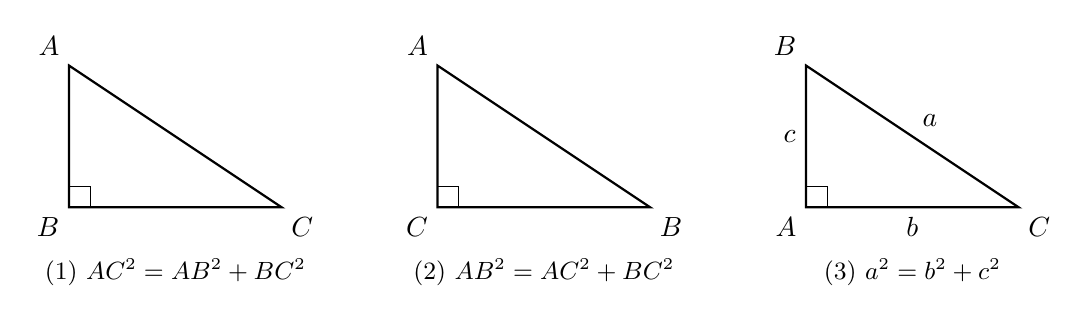
\begin{tikzpicture}[scale=0.9, >=latex]
  % (1) 角 B 為直角
  \begin{scope}[shift={(0,0)}]
    \coordinate (B) at (0,0);
    \coordinate (C) at (3,0);
    \coordinate (A) at (0,2);
    \draw[thick] (B) -- (C) -- (A) -- cycle;
    \draw (0,0.3) -- (0.3,0.3) -- (0.3,0);
    \node[below left] at (B) {$B$};
    \node[below right] at (C) {$C$};
    \node[above left] at (A) {$A$};
    \node[below=15pt] at (1.5,0) {\small (1) $AC^2 = AB^2 + BC^2$};
  \end{scope}

  % (2) 角 C 為直角
  \begin{scope}[shift={(5.2,0)}]
    \coordinate (C) at (0,0);
    \coordinate (B) at (3,0);
    \coordinate (A) at (0,2);
    \draw[thick] (C) -- (B) -- (A) -- cycle;
    \draw (0,0.3) -- (0.3,0.3) -- (0.3,0);
    \node[below left] at (C) {$C$};
    \node[below right] at (B) {$B$};
    \node[above left] at (A) {$A$};
    \node[below=15pt] at (1.5,0) {\small (2) $AB^2 = AC^2 + BC^2$};
  \end{scope}

  % (3) 角 A 為 90 度，邊長 a, b, c
  \begin{scope}[shift={(10.4,0)}]
    \coordinate (A) at (0,0);
    \coordinate (C) at (3,0);
    \coordinate (B) at (0,2);
    \draw[thick] (A) -- (C) node[midway, below] {$b$} -- (B) node[midway, above right] {$a$} -- cycle node[midway, left] {$c$};
    \draw (0,0.3) -- (0.3,0.3) -- (0.3,0);
    \node[below left] at (A) {$A$};
    \node[below right] at (C) {$C$};
    \node[above left] at (B) {$B$};
    \node[below=15pt] at (1.5,0) {\small (3) $a^2 = b^2 + c^2$};
  \end{scope}
\end{tikzpicture}
\caption{畢氏定理的幾種符號表示法對應圖}\label{fig:pythagoras_representations}
\end{figure}

上面三個表示法，都是正確的，並且顯然還有別的表示法。$\triangle$ 表示「三角形」，$A, B, C$ 表示三個平面上的點。$AC$ 表示「以 $A, C$ 為端點的一條線段」，並且顯然也表示了這條線段的長。這種區分在這裏並不是非常必要的，因為在這個問題裏，「線段」和「線段的長」並不需要確實區分。
\end{example}

在這門課中，我們還會遇到許多別的符號。大多數的符號，都會非常容易了解，但我們將在必要時，對所有的符號隨時加以說明。

\subsection*{習題 2-1}\label{sec:ex2-1}
\addcontentsline{toc}{subsection}{習題 2-1}

\begin{enumerate}[1., leftmargin=2em]
  \item 試以符號表示圓面積及圓周長之公式。
  \item 試以符號表示下面的敘述：\\
  「二相異正數之等差中項，必大於其等比中項。」
  \item 下面的一段文字中，有何不妥？請加以修改。\\
  「設 $a, b, c$ 為三線段的長，今以 $a, b, c$ 為三邊，作一三角形為 $\triangle ABC$。」
  \item 設有 $\triangle ABC$，試以符號表示下列各敘述：
  \begin{enumerate}[(i)]
    \item 它是直角三角形。
    \item 它是等腰三角形。
    \item 它是正三角形。
    \item 它是直角等腰三角形。
  \end{enumerate}
  \item 儘量以符號表示以下的定理（少用文字，多用符號）：
  \begin{enumerate}[(i)]
    \item 三角形中任意兩邊之和必大於第三邊。
    \item 三角形內角平分線交於一點，此點距此三角形之三邊等長。
  \end{enumerate}
  \item 令 $ABCD$ 為一個四邊形，試將下列各題中之符號用最簡明的文字敘述表示：
  \begin{enumerate}[(i)]
    \item $AB = CD$，$AD = BC$。
    \item $AB = CD$，$\angle DAC = 90^\circ$。
    \item $\angle A = \angle B = \angle C = \angle D = 90^\circ$。
    \item $AB = BC = CD = DA$，$\angle A = 90^\circ$。
    \item $\angle A = \angle B = \angle C = \angle D$，$AB = BC$。
    \item $AB = BC = CD = DA$。
    \item $\angle A + \angle C = 180^\circ$。
    \item $AB \parallel CD$。
  \end{enumerate}
  \item 試問下面的一段文字中，有何不妥？並作適當的修改。\\
  「設 $AB, CD$ 為二線段，將 $AB, CD$ 延長，令其交點為 $F$。」
  \item 試利用本節的方法，求 $879 + 654$ 之和，並解釋加法「逢十進位」的原理。同理，解釋 $782 + 978$ 和的「進位」原理。
  \item 觀察下列的平方數：
  \begin{align*}
    15^2 &= 225; & 25^2 &= 625; & 35^2 &= 1225; & 45^2 &= 2025; \\
    55^2 &= 3025; & 65^2 &= 4225; & 75^2 &= 5625; & 85^2 &= 7225; \\
    95^2 &= 9025; & 105^2 &= 11025; & \dots
  \end{align*}
  你能否發現到它們有一些共同規則嗎？（個位、十位的情形怎麼樣？百位以上的情形怎麼樣？）你能說明它們的理由嗎？\\
  〔提示：$(x+a)^2 = x^2 + 2ax + a^2$〕
  \item 推廣上題，考慮二數的乘積，如果這兩個數字的個位和為 $10$，十位以上之對應數字一一相同，像 $33 \times 37$，$42 \times 48$，$154 \times 156$，……那我們亦可得到類似上題之規則，請同學說明理由。\\
  〔提示：$(x+a)(x+b) = x^2 + (a+b)x + ab$〕
  \item[*] 觀察以下各數的平方：
  \begin{align*}
    11^2 &= 121; \\
    111^2 &= 12321; \\
    1111^2 &= 1234321; \dots \\
    (12345679 \times 9)^2 &= 12345678987654321.
  \end{align*}
  〔提示：$10 - 1 = 9$〕
\end{enumerate}

\subsection{集合}\label{sec:2-3}

\subsubsection*{甲、集合的概念}\label{subsec:2-3-a}

集合（set）是數學中很普遍的一個術語，一個集合是由它所含有的「元素」（element）（亦即組成單元）所湊集而成。譬如一條直線是由點所湊集成的集合，那些在這條直線上的點，就是該集合的元素。譬如在平面上，所有「和 $A$ 點的距離小於 $1$ 的點」成一集合，它所含的元素就是以 $A$ 點為圓心、$1$ 尺為半徑在平面上所畫的圓周以內的點（不包含圓周）。

\begin{figure}[htbp]
\centering
\begin{tikzpicture}[scale=1.1, >=latex]
  \draw[thick, dashed, fill=blue!10] (0,0) circle (1.5);
  \filldraw (0,0) circle (1.5pt) node[below] {$A$};
  \draw[->, thick] (0,0) -- (45:1.5) node[midway, above left] {$1$ 尺};
  \node at (0, 0.7) {\small 圓內部所有點組成的集合};
\end{tikzpicture}
\caption{平面上與 $A$ 點距離小於 $1$ 尺的點集示意}\label{fig:circle_interior_set}
\end{figure}

集合的概念是極簡單的，由一堆東西湊集而成的群體，就是一個集合。對於「一個集合」就數學的觀點而言，它只有一個要素：就是它所包含的那些「元素」。換句話說：\textbf{一個集合是由它所含有的元素完全決定！}（至於該集合各元素間是否具有相互關係？這些元素集成一個集合後是否有某種功效？從集合的觀念來說，是不相干的問題。）

在日常生活中，「集合」這個觀念是很普遍的。譬如某某學校的老師和同學們成一集合，你班上的同學們成一集合，你所在的教室中的桌椅成一集合，一隻錶的所有零件成一集合。但「集合的概念」只著重於其所含的「元素」，除此之外，沒有任何附帶涵義。一隻錶的零件，不論是將它們散放或者是將它們拼湊起來成為一隻能走的錶，由集合的觀點看來，都是同一集合，不加區分。

第一部集合論於公元 1878 年問世，由德國數學家康托（George Cantor, 1845--1918）所著。康托在書中解釋集合說：「集合是由明確而可鑑別的知覺對象或思維對象所聚合而成的，這些對象即稱為集合的元素。」

特別要請同學注意的是：\textbf{組成集合的元素必須明確可認定的}。譬如說：臺灣大學中文系漂亮的女生所成的集合，就很難確定。不說別的，李四覺得漂亮的，也許王二不以為然，在這情形下，達不成一致的規約，如何能定集合的元素呢？

\subsubsection*{乙、集合的描述}\label{subsec:2-3-b}

首先讓我們談一談集合的描述。

\begin{enumerate}[(一)]
  \item \textbf{列舉法}：假如一個集合 $A$ 只含有很少的幾個元素，則這個集合 $A$ 的一個最直截了當的表示法，就是把它所含的元素逐一列舉出來，通常我們再用括號 $\{\ \}$ 把列舉的元素括起來。
  
  \begin{example}\label{ex:2-3-1}
  \begin{enumerate}[(i)]
    \item $\{0, +1, -1\}$ 表示由 $0, +1, -1$ 三個元素所成的集合。
    \item $\{\triangle, \bigcirc, \square, \diamondsuit\}$ 表示由上述四個圖形所成的集合。
    \item $\{+, -, \times, \div\}$ 表示由 $+$, $-$, $\times$, $\div$ 四種運算符號所成的集合。
    \item $\{2, 3, 5, 7, 11, 13, 17, 19, 23, 29, 31, 37, 41, 43, 47, 53, 59, 61, 67, 71, 73, 79, 83, 89, 97\}$ 表示小於 $100$ 的二十五個正質數\footnote{\label{fn:prime}一個大於 $1$，而且除了 $1$ 和本身以外，不能被任何整數整除的數稱為「質數」，在第六章裏，我們將詳細討論它。}所成的集合。
  \end{enumerate}
  要注意的是：集合中括號內的元素可不顧順序，如
  \begin{align*}
    \{3, 7, 10\} &= \{10, 3, 7\} = \{7, 3, 10\}, \\
    \{\triangle, \bigcirc, \square, \diamondsuit\} &= \{\diamondsuit, \bigcirc, \square, \triangle\}.
  \end{align*}
  而且集合中同一元素書寫一次或多次，效果是一樣的，如
  \begin{align*}
    \{1, 2\} &= \{1, 2, 2, 2\}, \\
    \{2, 4, 6\} &= \{2, 2, 4, 6, 4, 6, 2\}, \\
    \{p, p, q, r\} &= \{p, q, r\}.
  \end{align*}
  \end{example}

  \item \textbf{特徵性質描述法}：從上面的最後一個例子，同學們可以看出當該集合的元素稍多一些的時候，逐一列舉的描述法是很煩瑣而不經濟的。另一種最常用的描述方法是：用該集合所含的元素的「特徵性質」去描述它。這種方法，我們以前已經用過，現在再舉例如下：
  
  \begin{example}\label{ex:2-3-2}
  \begin{enumerate}[(i)]
    \item 「偶數全體所成的集合」，「所有能被 $2$ 整除的整數所成的集合」，都是用來描述一個元素為 $0, \pm 2, \pm 4, \pm 6, \dots$ 的集合。
    \item 同樣地，「奇數全體所成的集合」，「所有不能被 $2$ 整除的整數所成的集合」，都是用來描述一個元素為 $\pm 1, \pm 3, \pm 5, \dots$ 的集合。
    \item 在平面 $P$ 上，一個以 $O$ 點為圓心、$1$ 尺為半徑的圓內的點所成的集合，也可以用「所有和 $O$ 點的距離小於 $1$ 尺的點所成的集合」去加以描述。
    \item $\{+\sqrt{2}, -\sqrt{2}\}$ 這一集合也可描述為「其平方為 $2$ 的數所成的集合」。
    \item 所有絕對值小於或等於 $1$ 的實數成一集合。
  \end{enumerate}
  \end{example}

  以上這種描述法是我們常用的。在本章第一節中我們曾一再強調數學符號的第一要素就是明確。所以在我們用「某一性質」去描述一個集合時，該性質一定要絕對明確；譬如：「大於 $100000$」是一個明確的性質，但是「相當大」就不是一個明確的性質。所以假如你隨隨便便說：「$A$ 是由相當大的有理數所成的集合」，別人一定會問究竟大到什麼程度才叫相當大？

  \item \textbf{典型元素描述法}：假如我們把列舉法與特徵性質法適當地加以配合，我們可以把集合所含的「典型元素」（typical element）加以描述。現在將例~\ref{ex:2-3-2} 中的五個例子，依次描述如下：
  \begin{enumerate}[(i)]
    \item $A = \{2n \mid n \text{ 為任意整數}\} = \{x \mid x \text{ 為整數，且能被 } 2 \text{ 整除}\}$。如以 $\mathbb{Z}$ 表示所有整數的集合，則又可寫成 $A = \{2n \mid n \in \mathbb{Z}\}$。
    \item $B = \{2n+1 \mid n \text{ 為任意整數}\} = \{x \mid x \text{ 為整數，且不能被 } 2 \text{ 整除}\} = \{2n+1 \mid n \in \mathbb{Z}\}$。
    \item $C = \{X \mid X \in P, OX \text{ 的長度} < 1 \text{ 尺}\}$。
    \item $D = \{x \mid x^2 = 2\}$。
    \item $E = \{x \mid |x| \le 1\}$。
  \end{enumerate}
  以上這種描述法在數學中是最常用的描述法，它和特徵性質描述法是很類似的。事實上，它就是把特徵性質描述法用適當的符號表示出來。
\end{enumerate}

\subsubsection*{丙、集合的記號}\label{subsec:2-3-c}

\begin{enumerate}[(一)]
  \item \textbf{屬於}：\\
  我們用符號「$\in$」表示「屬於」。式子
  \begin{equation}\label{eq:belong_rel}
    a \in B
  \end{equation}
  表示 $a$ 是集合 $B$ 的一個元素，讀做「$a$ 屬於 $B$」。譬如我們以 $A$ 表示所有絕對值大於 $1$ 的有理數所成的集合，則有：
  \begin{equation*}
    2 \in A, \quad -5 \in A, \quad \pm \frac{7}{2} \in A, \quad \frac{23}{3} \in A, \quad \dots \text{ 等等}。
  \end{equation*}
  相對地，我們用符號「$\notin$」表示「不屬於」。以上述集合 $A$ 為例，我們有：
  \begin{equation*}
    0 \notin A, \quad 1 \notin A, \quad -1 \notin A, \quad \frac{1}{2} \notin A, \quad -\frac{3}{5} \notin A, \quad \dots \text{ 等等}。
  \end{equation*}

  \item \textbf{子集}：\\
  假如集合 $A$ 的任一元素都一定也是集合 $B$ 的元素，我們就說 $A$ 是 $B$ 的一個「\textbf{子集}」。也可以說 $A$「包含於」$B$，或 $B$「包含」$A$，我們以符號
  \begin{equation}\label{eq:subset_rel}
    A \subseteq B \quad \text{或} \quad B \supseteq A
  \end{equation}
  表示之。要注意的是，按照上述定義，一個集合 $A$ 也是它本身的子集，亦即 $A \subseteq A$\footnote{\label{fn:subset_self}註：我們說明一下為什麼 $A \subseteq A$。讓我們看一看什麼叫做「$\subseteq$」：$A \subseteq B$ 的定義是：$A$ 中任一元素都一定是 $B$ 中某一元素。因此，$A \subseteq C$ 的定義是：$A$ 中任一元素都一定是 $C$ 中某一元素。因為上面的 $C$ 是可以變換的，假如我們把它變成 $A$，那麼 $A \subseteq A$ 的定義是：$A$ 中任一元素都一定也是 $A$ 中某一元素。這句話當然是對的（想一想：你班上的任一個同學，是不是你班上的某一個同學？）。因此，我們才可以說：由於「$\subseteq$」的定義，而且由於 $A$ 和 $A$ 之間滿足了這項定義，所以便有 $A \subseteq A$。有的書上把記號 $\subseteq$ 簡寫成 $\subset$，請同學在閱讀推演時先認清所用的符號。}。

  \begin{example}\label{ex:2-3-3}
  設：
  \begin{itemize}
    \item $A$ 是絕對值大於 $1$ 的有理數所成的集合，
    \item $B$ 是絕對值大於 $\frac{1}{3}$ 的有理數所成的集合，
    \item $C$ 是不等於 $0$ 的有理數所成的集合，
    \item $D$ 是大於 $1$ 的有理數所成的集合，
  \end{itemize}
  則上述四個集合間，有下述關係：
  \begin{equation*}
    A \subseteq B, \quad A \subseteq C, \quad B \subseteq C, \quad D \subseteq B, \quad D \subseteq C, \quad D \subseteq A,
  \end{equation*}
  且 $A \subseteq A, B \subseteq B, C \subseteq C, D \subseteq D$。
  \end{example}

  集合之間的關係，我們常以直觀而簡單的圖形表示。上面例子中 $A, B, C, D$ 四集合之間的關係，就可以用下面的圖形表示出來：

  \begin{figure}[htbp]
  \centering
  \begin{tikzpicture}[scale=0.9, >=latex]
    \draw[thick] (0,0) circle (3.2) node[below=2.6cm] {$C$（非零有理數）};
    \draw[thick] (0,0.3) circle (2.2) node[below=1.6cm] {$B$（$|x| > 1/3$）};
    \draw[thick] (0,0.6) circle (1.3) node[below=0.8cm] {$A$（$|x| > 1$）};
    \draw[thick] (0,1.1) circle (0.6) node {$D$（$x > 1$）};
  \end{tikzpicture}
  \caption{集合包含關係 $D \subseteq A \subseteq B \subseteq C$ 示意圖}\label{fig:nested_subsets}
  \end{figure}

  同學們不難從定義看出：「假如 $A$ 是 $B$ 的子集，$B$ 是 $C$ 的子集，則 $A$ 也是 $C$ 的子集。」亦即：
  \begin{equation}\label{eq:transitive_subset}
    \text{假如 } A \subseteq B, \ B \subseteq C, \text{ 則 } A \subseteq C,
  \end{equation}
  以圖表示如下：

  \begin{figure}[htbp]
  \centering
  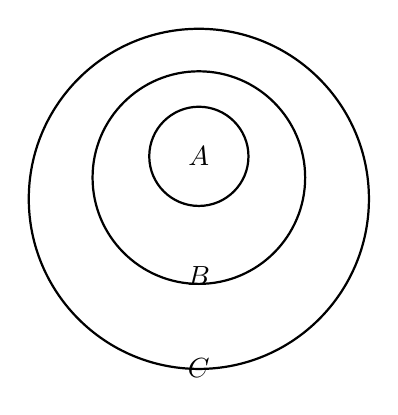
\begin{tikzpicture}[scale=0.9, >=latex]
    \draw[thick] (0,0) circle (2.4) node[below=1.9cm] {$C$};
    \draw[thick] (0,0.3) circle (1.5) node[below=1.0cm] {$B$};
    \draw[thick] (0,0.6) circle (0.7) node {$A$};
  \end{tikzpicture}
  \caption{子集關係的遞移性：$A \subseteq B$ 且 $B \subseteq C \implies A \subseteq C$}\label{fig:transitive_subset}
  \end{figure}

  \item \textbf{聯集與交集}：\\
  把集合 $A$ 的所有元素和集合 $B$ 的所有元素合併而成的集合叫做「\textbf{集合 $A, B$ 的聯集}」，以符號
  \begin{equation}\label{eq:union_def}
    A \cup B
  \end{equation}
  表示之。由一個集合 $A$ 和一個集合 $B$ 的公共元素所成的集合叫做「\textbf{集合 $A, B$ 的交集}」，以符號
  \begin{equation}\label{eq:intersection_def}
    A \cap B
  \end{equation}
  表示之。

  \begin{example}\label{ex:2-3-4}
  設 $A = \{1, 2\}$，$B = \{2, 3\}$，那麼：
  \begin{equation*}
    A \cup B = \{1, 2, 3\}, \qquad A \cap B = \{2\}。
  \end{equation*}
  \end{example}

  \begin{example}\label{ex:2-3-5}
  設 
  \begin{align*}
    A &= \{x \mid x \text{ 是實數，} -7 < x < 5\}, \\
    B &= \{x \mid x \text{ 是實數，} -3 < x < 10\},
  \end{align*}
  那麼
  \begin{align*}
    A \cup B &= \{x \mid x \text{ 是實數，} -7 < x < 10\}, \\
    A \cap B &= \{x \mid x \text{ 是實數，} -3 < x < 5\}。
  \end{align*}
  像 $A, B$ 這樣的集合，通常用符號
  \begin{equation*}
    A = (-7, 5), \qquad B = (-3, 10)
  \end{equation*}
  表示，稱為\textbf{開區間}。

  \begin{figure}[htbp]
  \centering
  \begin{tikzpicture}[scale=0.75, >=latex]
    \draw[->, thick] (-9, 0) -- (12, 0) node[right] {實數線};
    \foreach \x in {-8, -6, ..., 10} {
      \draw (\x, 0.15) -- (\x, -0.15) node[below] {\footnotesize \x};
    }
    % 區間 A: (-7, 5)
    \draw[thick, blue] (-7, 0.8) -- (5, 0.8);
    \draw[blue, fill=white] (-7, 0.8) circle (3pt);
    \draw[blue, fill=white] (5, 0.8) circle (3pt);
    \node[left, blue] at (-7, 0.8) {$A = (-7, 5)$};

    % 區間 B: (-3, 10)
    \draw[thick, red] (-3, 1.6) -- (10, 1.6);
    \draw[red, fill=white] (-3, 1.6) circle (3pt);
    \draw[red, fill=white] (10, 1.6) circle (3pt);
    \node[left, red] at (-3, 1.6) {$B = (-3, 10)$};

    % 交集 A cap B
    \draw[very thick, purple] (-3, 0) -- (5, 0);
    \draw[purple, fill=white] (-3, 0) circle (3pt);
    \draw[purple, fill=white] (5, 0) circle (3pt);
    \node[above, purple] at (1, 0.15) {\small $A \cap B = (-3, 5)$};
  \end{tikzpicture}
  \caption{開區間的聯集與交集在實數線上之圖解}\label{fig:open_intervals}
  \end{figure}
  \end{example}

  \begin{example}\label{ex:2-3-6}
  設 
  \begin{align*}
    C &= \{x \mid x \text{ 是實數，} -2 \le x \le 6\}, \\
    D &= \{x \mid x \text{ 是實數，} -4 \le x \le 3\},
  \end{align*}
  則
  \begin{align*}
    C \cup D &= \{x \mid x \text{ 是實數，} -4 \le x \le 6\} = [-4, 6], \\
    C \cap D &= \{x \mid x \text{ 是實數，} -2 \le x \le 3\} = [-2, 3]。
  \end{align*}
  如例~\ref{ex:2-3-5}，可用符號 $C = [-2, 6]$，$D = [-4, 3]$ 表示，稱為\textbf{閉區間}。一般來說，稱 $\{x \mid x \text{ 是實數，} a < x < b\}$ 為開區間，記為 $(a, b)$；而 $\{x \mid x \text{ 是實數，} a \le x \le b\}$ 稱為閉區間，記為 $[a, b]$。
  \end{example}

  \begin{example}\label{ex:2-3-7}
  設 $A$ 是下圖圓形中的點所成的集合，$B$ 是方形中的點所成的集合，則 $A \cup B$ 是左下圖中有斜線部分的點所成的集合，$A \cap B$ 是右下圖中有斜方格部分的點所成的集合。

  \begin{figure}[htbp]
  \centering
  \begin{minipage}[t]{0.45\textwidth}
  \centering
  \begin{tikzpicture}[scale=0.85]
    \fill[pattern=north east lines, pattern color=blue!60] (-0.8, 0) circle (1.3);
    \fill[pattern=north east lines, pattern color=blue!60] (0.2, -1.1) rectangle (2.2, 0.9);
    \draw[thick] (-0.8, 0) circle (1.3) node[left=18pt] {$A$};
    \draw[thick] (0.2, -1.1) rectangle (2.2, 0.9) node[right=18pt] {$B$};
    \node[below=15pt] at (0.6, -1.1) {\small 聯集 $A \cup B$（斜線部分）};
  \end{tikzpicture}
  \end{minipage}
  \hfill
  \begin{minipage}[t]{0.45\textwidth}
  \centering
  \begin{tikzpicture}[scale=0.85]
    \begin{scope}
      \clip (-0.8, 0) circle (1.3);
      \fill[pattern=grid, pattern color=red!70] (0.2, -1.1) rectangle (2.2, 0.9);
    \end{scope}
    \draw[thick] (-0.8, 0) circle (1.3) node[left=18pt] {$A$};
    \draw[thick] (0.2, -1.1) rectangle (2.2, 0.9) node[right=18pt] {$B$};
    \node[below=15pt] at (0.6, -1.1) {\small 交集 $A \cap B$（網格部分）};
  \end{tikzpicture}
  \end{minipage}
  \caption{幾何圖形點集的聯集與交集示意}\label{fig:geom_union_intersection}
  \end{figure}
  \end{example}

  從兩種集合 $A, B$ 得出它們的「聯集」與「交集」是很自然、很簡單的兩種運算。但是當 $A, B$ 兩集合不含任何公共元素時，如下圖所示：

  \begin{figure}[htbp]
  \centering
  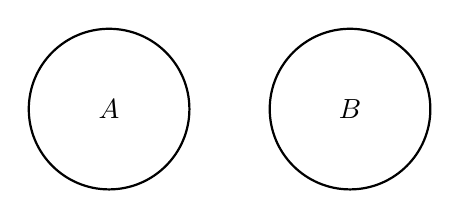
\begin{tikzpicture}[scale=0.85]
    \draw[thick] (-1.8, 0) circle (1.2) node {$A$};
    \draw[thick] (1.8, 0) circle (1.2) node {$B$};
  \end{tikzpicture}
  \caption{兩不相交集合示意}\label{fig:disjoint_sets}
  \end{figure}

  交集 $A \cap B$ 的意義是什麼呢？這裏我們只有兩種說法可供選擇：
  \begin{enumerate}[(i)]
    \item 我們可以在交集的定義中申明：當 $A, B$ 兩集合不含任何公共元素時，「$A, B$ 的交集」沒有意義，所以符號「$A \cap B$」也沒有意義。換句話說，$A \cap B$ 這個符號僅在 $A, B$ 有公共元素時，才能使用。
    \item 另外一種辦法是：引入一個特殊的「集合」，它不含任何元素，叫做「\textbf{空集合}」。然後說：當 $A, B$ 兩集合不含任何公共元素時，「$A, B$ 的交集」就是「空集合」。通常我們約定以符號「$\emptyset$」表示「空集合」，而上述事實用符號
    \begin{equation}\label{eq:disjoint_empty}
      A \cap B = \emptyset
    \end{equation}
    表示之。
  \end{enumerate}
  對於上述兩種辦法的取捨，自然得看哪一種辦法用起來較為方便簡明。經試用的結果，發現第二種辦法遠較第一種辦法簡潔易用，這也就是我們引入「空集合」這個特殊的集合的原因。

  \begin{example}\label{ex:2-3-8}
  奇數集合 $\cap$ 偶數集合 $= \emptyset$。
  \end{example}

  \begin{example}\label{ex:2-3-9}
  設 $A = \{x \mid x \text{ 為實數，} x > 0\}$，$B = \{x \mid x \text{ 為實數，} x < 0\}$，則 $A \cap B = \emptyset$。
  \end{example}
\end{enumerate}

\subsection*{習題 2-2}\label{sec:ex2-2}
\addcontentsline{toc}{subsection}{習題 2-2}

\begin{enumerate}[1., leftmargin=2em]
  \item 設 $\mathbb{N}$ 為所有自然數的集合，$\mathbb{Z}$ 為所有整數的集合，$\mathbb{Q}$ 為所有有理數的集合，$\mathbb{R}$ 為所有實數的集合，下列各數各屬於或不屬於哪些集合？用符號寫出。
  \begin{equation*}
    -3, \quad 0, \quad 1, \quad 2, \quad \frac{1+\sqrt{5}}{2}, \quad \frac{3}{7}, \quad -\frac{3}{4}, \quad 14。
  \end{equation*}
  \item 把下列各集合以第三種典型元素描述法寫出來，儘量運用符號：
  \begin{enumerate}[(i)]
    \item 平面 $P$ 上，以 $O$ 為圓心、$r$ 為半徑的圓周上的點。
    \item $A = \{1, 3, 5, 7, 9, 11, 13, 15, 17, 19\}$；$B = \{2, 4, 6, 8, 10, 12, 14, 16, 18, 20\}$；$C = \{7, 14, 21, 28, 35, 42\}$。
    \item 所有加上 $7$ 就大於 $15$ 的實數。
    \item 所有平方後就大於 $7$ 的實數。
  \end{enumerate}
  \item 設 $A$ 是所有平方數的集合，$B$ 是所有立方數的集合，將 $A, B$ 及 $A \cap B$ 以典型元素描述法寫出來。
  \item 下列集合中哪些是空集合？哪些只包含一個元素？
  \begin{align*}
    S_1 &= \{p \mid p \text{ 為質數，且 } 890 < p < 900\}, \\
    S_2 &= \{p \mid p \in \mathbb{N}, \ p \text{ 為可被 } 29 \text{ 整除的質數}\}, \\
    S_3 &= \{n \mid n \in \mathbb{N}, \text{ 且 } 3^n + 4^n = 5^n\}。
  \end{align*}
  \item 下列諸題中，判定 $A, B$ 二集合之關係：
  \begin{enumerate}[(i)]
    \item $A = \{x \mid 2x+4 \ge x-5\}$，$B = \{x \mid 3x+5 \ge 2x-4\}$。
    \item $A = \{x \mid x^2 + 4 = -2x+2\}$，$B = \{x \mid x^2 + 2x \le -2\}$。
    \item $A = \{x \mid a \le x \le b\}$，$B = \{y \mid 2a \le y \le 2b\}$，設 $a < 0 < b$。
    \item $A = \{x \mid x \text{ 為一等腰三角形}\}$，$B = \{y \mid y \text{ 為一等腰三角形}\}$。
    \item $A = \{a_i \mid i=1, 2, \dots, n\}$，$B = \{a_k \mid k=1, 2, 3, \dots, n+6\}$，$n \ge 1$。
    \item $A = \{x \mid x \text{ 是等腰三角形}\}$，$B = \{x \mid x \text{ 是正三角形}\}$。
  \end{enumerate}
  \item 把下列各集合寫成 $A \cap B$ 的型式，使 $A \nsubseteq B, B \nsubseteq A$，$A, B$ 都以典型方法表示：
  \begin{enumerate}[(i)]
    \item 所有大於 $3$ 小於 $5$ 的數。
    \item 所有正方形。〔提示：正方形為四邊等、四角相等的四邊形〕
    \item $12, 18$ 的最小公倍數的倍數。
    \item $\{P \mid OP = 5\}$（一切點都在一平面內）。
  \end{enumerate}
  \item 把下列各集合寫成 $A \cup B$ 之型式，且使 $A \nsubseteq B, B \nsubseteq A$：
  \begin{enumerate}[(i)]
    \item 所有不為 $3$ 除盡的整數。
    \item 所有的實數。
    \item 所有絕對值大於 $1$ 的實數。
  \end{enumerate}
  \item 設 $A$ 為所有四邊形的集合，$B$ 為所有梯形的集合，$C$ 為所有平行四邊形的集合，$D$ 為所有菱形的集合，$E$ 為所有長方形的集合，$F$ 為所有正方形的集合。以圖形表示下列各集合間之關係：
  \begin{enumerate}[(i)]
    \item $A, B, C, E, F$。
    \item $A, D, E, F$。
    \item $A, B, C, D, E, F$。
  \end{enumerate}
  \item 設 $A$ 為所有三角形的集合，$A_{90}$ 為所有直角三角形的集合，$B_2$ 為所有等腰三角形的集合，$B_3$ 為所有等邊三角形的集合，$A_{60}$ 為所有三角形中至少有一角為 $60^\circ$ 者所成的集合。
  \begin{enumerate}[(i)]
    \item 用圖形表示這些集合的關係。
    \item $A_{90} \cap B_3 = ?$
  \end{enumerate}
  \item 設 $A, B$ 表示二集合，試證：
  \begin{enumerate}[(i)]
    \item $A \subseteq A \cup B, \quad B \subseteq A \cup B$。
    \item $A \supseteq A \cap B, \quad B \supseteq A \cap B$。
    \item 設 $A \subseteq B$，而 $H$ 為任意集合，則 $A \cup H \subseteq B \cup H$。
    \item 設 $A \subseteq B$，而 $H$ 為任意集合，則 $A \cap H \subseteq B \cap H$。
    \item $A \cup (A \cap B) = A$。
    \item $B \cap (A \cup B) = B$。
  \end{enumerate}
  \item[*] 試證 $D = A \cap B$ 滿足下列兩性質：
  \begin{enumerate}[(1)]
    \item $D \subseteq A, \ D \subseteq B$。
    \item 滿足 $E \subseteq A, \ E \subseteq B$ 的任一集合 $E$，必定包含於 $D$。
  \end{enumerate}
  \item[*] 試證任一集合 $D$ 若滿足下列二性質：
  \begin{enumerate}[(1)]
    \item $D \subseteq A, \ D \subseteq B$。
    \item 滿足 $E \subseteq A, \ E \subseteq B$ 的任一集合 $E$，必定包含於 $D$。
  \end{enumerate}
  則此集合 $D$ 即為 $A \cap B$。
  \item[*] 試證 $C = A \cup B$ 滿足下二性質：
  \begin{enumerate}[(1)]
    \item $C \supseteq A, \ C \supseteq B$。
    \item 滿足 $F \supseteq A$ 且 $F \supseteq B$ 的任一集合 $F$，必定包含 $C$。
  \end{enumerate}
  \item[*] 試證任一集合 $C$ 若滿足下二性質：
  \begin{enumerate}[(1)]
    \item $C \supseteq A, \ C \supseteq B$。
    \item 滿足 $F \supseteq A$ 且 $F \supseteq B$ 的任一集合 $F$，必定包含 $C$。
  \end{enumerate}
  則此集合 $C$ 即為 $A \cup B$。
\end{enumerate}

\subsubsection*{丁、集合的差}\label{subsec:2-3-d}

對於集合 $A, B$，我們定義 $A, B$ 之間的「\textbf{差}」如下：
\begin{align*}
  A \setminus B &\text{ 是由所有「屬於 $A$ 但是不屬於 $B$」的元素所成的集合}； \\
  B \setminus A &\text{ 是由所有「屬於 $B$ 但是不屬於 $A$」的元素所成的集合}。
\end{align*}

\begin{figure}[htbp]
\centering
\begin{minipage}[t]{0.45\textwidth}
\centering
\begin{tikzpicture}[scale=0.85]
  \begin{scope}
    \clip (-0.8, 0) circle (1.3);
    \fill[pattern=north east lines, pattern color=blue!60] (-0.8, 0) circle (1.3);
  \end{scope}
  \fill[white] (0.2, -1.1) rectangle (2.2, 0.9);
  \draw[thick] (-0.8, 0) circle (1.3) node[left=18pt] {$A$};
  \draw[thick] (0.2, -1.1) rectangle (2.2, 0.9) node[right=18pt] {$B$};
  \node[below=15pt] at (0.6, -1.1) {\small 差集 $A \setminus B$};
\end{tikzpicture}
\end{minipage}
\hfill
\begin{minipage}[t]{0.45\textwidth}
\centering
\begin{tikzpicture}[scale=0.85]
  \begin{scope}
    \clip (0.2, -1.1) rectangle (2.2, 0.9);
    \fill[pattern=north west lines, pattern color=red!60] (0.2, -1.1) rectangle (2.2, 0.9);
  \end{scope}
  \fill[white] (-0.8, 0) circle (1.3);
  \draw[thick] (-0.8, 0) circle (1.3) node[left=18pt] {$A$};
  \draw[thick] (0.2, -1.1) rectangle (2.2, 0.9) node[right=18pt] {$B$};
  \node[below=15pt] at (0.6, -1.1) {\small 差集 $B \setminus A$};
\end{tikzpicture}
\end{minipage}
\caption{集合之差 $A \setminus B$ 與 $B \setminus A$ 示意}\label{fig:set_difference}
\end{figure}

\begin{example}\label{ex:2-3-10}
設 $A = \{1, 3, 5, 7\}$，$B = \{3, 7, 11\}$，$C = \{3, 9, 13\}$。則：
\begin{align*}
  A \setminus B &= \{1, 5\}, & A \setminus C &= \{1, 5, 7\}, \\
  B \setminus A &= \{11\}, & C \setminus A &= \{9, 13\}, \\
  B \setminus C &= \{7, 11\}, & C \setminus B &= \{9, 13\}。
\end{align*}
\end{example}

\begin{example}\label{ex:2-3-11}
設 $A = \text{直角三角形集合}$，$B = \text{等腰三角形集合}$。那麼 $A \setminus B$ 是「非等腰的直角三角形集合」，而 $B \setminus A$ 是「非直角的等腰三角形集合」。
\end{example}

\begin{example}\label{ex:2-3-12}
由一個實驗的結果造成的集合。

假如我們擲一個骰子兩次，而將它們可能的結果記錄下來，便有 $36$ 種可能的情形：
\begin{equation*}
\begin{array}{cccccc}
  (1, 1), & (1, 2), & (1, 3), & (1, 4), & (1, 5), & (1, 6), \\
  (2, 1), & (2, 2), & (2, 3), & (2, 4), & (2, 5), & (2, 6), \\
  \dots & & & & & \\
  (6, 1), & (6, 2), & (6, 3), & (6, 4), & (6, 5), & (6, 6)
\end{array}
\end{equation*}
〔$(3, 2)$ 表示第一次得 $3$，第二次得 $2$〕。令 $W$ 為以上 $36$ 種情形所成的集合，那麼許多「事件」便可以用子集表示出來。

例如：「第一次得 $5$」這一件「事」，便可由
\begin{equation*}
  A = \{(5, 1), (5, 2), (5, 3), (5, 4), (5, 5), (5, 6)\}
\end{equation*}
表示；而「兩次點數之和為 $7$」可以用
\begin{equation*}
  B = \{(1, 6), (2, 5), (3, 4), (4, 3), (5, 2), (6, 1)\}
\end{equation*}
表示。

而 $A \cap B$ 表示「第一次得 $5$ 而且兩次之和為 $7$」，我們可以看出，第二次的結果非 $2$ 不可，因此：
\begin{equation*}
  A \cap B = \{(5, 2)\}。
\end{equation*}
如果我們直接觀察 $A, B$ 兩個集合，發現 $(5, 2)$ 是它們唯一的共同元素，這樣也得到上面相同的結果。

此外我們還有：
\begin{itemize}
  \item $W \setminus A =$「第一次不得 $5$」；
  \item $W \setminus B =$「二次之和不得為 $7$」；
  \item $A \cup B =$「第一次得 $5$，或者兩次的和為 $7$」；
  \item $A \setminus B =$「第一次得 $5$，但第二次不得為 $2$」。
\end{itemize}
\end{example}

\subsubsection*{戊、集合運算法則}\label{subsec:2-3-e}

在上面一段中，我們引入下列有關集合的符號：
\begin{itemize}
  \item $\in$：屬於；如「$b \in A$」讀成「$b$ 屬於 $A$」。
  \item $\supseteq$：包含；如「$B \supseteq A$」讀成「$B$ 包含 $A$」。
  \item $\subseteq$：包含於；如「$A \subseteq B$」讀成「$A$ 包含於 $B$」。
  \item $\cap$：交集運算；如「$A \cap B$」讀成「$A, B$ 的交集」。
  \item $\emptyset$：空集合。
  \item $\cup$：聯集運算；如「$A \cup B$」讀成「$A, B$ 的聯集」。
  \item $\setminus$：差；如「$A \setminus B$」讀成「$A, B$ 之差」，「$B \setminus A$」讀成「$B, A$ 之差」。
\end{itemize}

注意：
\begin{enumerate}[(i)]
  \item 「$A, B$ 之差」和「$B, A$ 之差」是不同的兩個集合。
  \item 「$\in$」是元素和集合之間的關係，但是「$\supseteq$」和「$\subseteq$」是集合和集合之間的關係，後者有“比較”的意味在內。
\end{enumerate}

上述「運算」或「符號」之間具有很多有用的相互關連，現在說明如下：

\begin{enumerate}[(i)]
  \item 我們規定「空集合」$\emptyset$ 是任何集合的子集，亦即 $\emptyset \subseteq A$ 對任何集合 $A$ 皆成立。
  \begin{example}\label{ex:2-3-13}
  設集合 $A = \{1, 2, 3\}$，那麼 $A$ 的子集共有下列八個：
  \begin{equation*}
    \{1, 2, 3\}, \quad \{1, 2\}, \quad \{2, 3\}, \quad \{1, 3\}, \quad \{1\}, \quad \{2\}, \quad \{3\}, \quad \emptyset。
  \end{equation*}
  \end{example}

  \item 「$A \subseteq B$ 且 $B \subseteq A$」和「$A = B$」是一回事。
  \begin{example}\label{ex:2-3-14}
  設 $A$ 為所有三邊相等的三角形的集合，$B$ 為所有三個角相等的三角形的集合。當然，$A = B$。
  
  讓我們想一想為什麼 $A = B$：這是因為三邊相等的三角形，一定三個角也相等。亦即任一個 $A$ 中元素，也必都是 $B$ 中之元素，所以 $A \subseteq B$。反過來看，三個角都相等的三角形，一定也三邊相等。因此，任何 $B$ 中之元素，必也是 $A$ 中之元素，所以 $B \subseteq A$。有了這些了解，我們當然看出 $A$ 和 $B$ 非是同樣的集合不可，因為 $A$ 和 $B$ 中的元素都是「正三角形」，而一個集合又是完全被它所包含的元素決定的。
  
  一般說來，我們要證明二個集合 $A$ 和 $B$ 相等時，一個典型的方法就是先證明 $A \subseteq B$，再證明 $B \subseteq A$。這是因為由這裏可直接查核 $A, B$「是不是同一個集合」，而在另一面，「包含」的關係比較容易驗證。
  \end{example}

  \item 包含關係的多種等價描述：
  \begin{align*}
    \text{「} A \supseteq B \text{」和「} A \cap B = B \text{」是一回事}； \\
    \text{「} A \supseteq B \text{」和「} A \cup B = A \text{」也是一回事}； \\
    \text{「} A \supseteq B \text{」和「} B \setminus A = \emptyset \text{」也是一回事}。
  \end{align*}
  同學們請自行作圖驗證之。

  \item \textbf{交集運算的結合律}：
  \begin{equation}\label{eq:assoc_intersection}
    (A \cap B) \cap C = A \cap (B \cap C) = A \cap B \cap C,
  \end{equation}
  因為它們都是由 $A, B, C$ 的所有公共元素所成的集合。

  \item \textbf{聯集運算的結合律}：
  \begin{equation}\label{eq:assoc_union}
    (A \cup B) \cup C = A \cup (B \cup C) = A \cup B \cup C,
  \end{equation}
  因為它們都是把所有 $A, B, C$ 的元素合併而成的集合。

  \item \textbf{集合運算的分配律}：
  \begin{align}
    A \cap (B \cup C) &= (A \cap B) \cup (A \cap C), \label{eq:dist_cap_over_cup} \\
    A \cup (B \cap C) &= (A \cup B) \cap (A \cup C)。 \label{eq:dist_cup_over_cap}
  \end{align}

  \item \textbf{笛摩根定理}（De Morgan's Laws）：
  \begin{align}
    A \setminus (B \cup C) &= (A \setminus B) \cap (A \setminus C), \label{eq:demorgan_diff_cup} \\
    A \setminus (B \cap C) &= (A \setminus B) \cup (A \setminus C)。 \label{eq:demorgan_diff_cap}
  \end{align}
  上述 (vi), (vii) 兩點的理由我們留待下節再加說明，但是其大意可以從下圖清楚地看出：

  \begin{figure}[htbp]
  \centering
  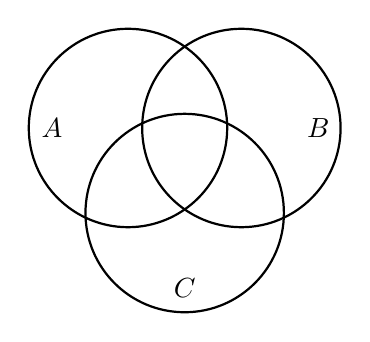
\begin{tikzpicture}[scale=0.9]
    \draw[thick] (-0.8, 0.5) circle (1.4) node[left=20pt] {$A$};
    \draw[thick] (0.8, 0.5) circle (1.4) node[right=20pt] {$B$};
    \draw[thick] (0, -0.7) circle (1.4) node[below=20pt] {$C$};
  \end{tikzpicture}
  \caption{三集合分配律與笛摩根定理文氏圖解析}\label{fig:venn_three_sets}
  \end{figure}

  請同學對上述三個集合 $A, B, C$ 逐一檢驗 (vi)、(vii) 中四個等式中所出現的每一集合，這對於上述等式的瞭解是很有幫助的。

  \begin{example}\label{ex:2-3-15}
  設 $A = \{1, 2, 3\}$，$B = \{2, 3, 4, 5\}$，$C = \{3, 5, 6\}$。
  \begin{itemize}
    \item 由於 $B \cup C = \{2, 3, 4, 5, 6\}$，$A \cap (B \cup C) = \{2, 3\}$。又 $A \cap B = \{2, 3\}$，$A \cap C = \{3\}$，$(A \cap B) \cup (A \cap C) = \{2, 3\}$。所以
    \begin{equation*}
      A \cap (B \cup C) = (A \cap B) \cup (A \cap C)。
    \end{equation*}
    \item 又因為 $B \cap C = \{3, 5\}$，$A \cup (B \cap C) = \{1, 2, 3, 5\}$。且 $A \cup B = \{1, 2, 3, 4, 5\}$，$A \cup C = \{1, 2, 3, 5, 6\}$，$(A \cup B) \cap (A \cup C) = \{1, 2, 3, 5\}$。所以
    \begin{equation*}
      A \cup (B \cap C) = (A \cup B) \cap (A \cup C)。
    \end{equation*}
  \end{itemize}
  \end{example}

  \begin{example}\label{ex:2-3-16}
  我們仍考慮例~\ref{ex:2-3-15} 中的 $A, B, C$：
  \begin{itemize}
    \item 因為 $A \setminus (B \cup C) = \{1\}$；又 $A \setminus B = \{1\}$，$A \setminus C = \{1, 2\}$，$(A \setminus B) \cap (A \setminus C) = \{1\}$。所以
    \begin{equation*}
      A \setminus (B \cup C) = (A \setminus B) \cap (A \setminus C)。
    \end{equation*}
    \item 又因為 $A \setminus (B \cap C) = \{1, 2\}$，且 $(A \setminus B) \cup (A \setminus C) = \{1, 2\}$。所以
    \begin{equation*}
      A \setminus (B \cap C) = (A \setminus B) \cup (A \setminus C)。
    \end{equation*}
  \end{itemize}
  \end{example}
\end{enumerate}

\subsubsection*{己、性質與集合的關係及元素個數計算}\label{subsec:2-3-f}

在上面我們提及可以用性質去描述一個集合，所以對於一個集合，我們也可以去討論它的元素所具有的共同性質。

譬如 $A$ 是所有具有性質 $\alpha$ 的元素所成的集合，$B$ 是所有具有性質 $\beta$ 的元素所成的集合，則：
\begin{itemize}
  \item $A \cap B$ 就是所有具有性質 $\alpha$ 和 $\beta$ 的元素所成的集合；
  \item $A \cup B$ 就是所有具有性質 $\alpha$ 或 $\beta$ 的元素所成的集合；
  \item $A \setminus B$ 是那些具有性質 $\alpha$，但是不具有性質 $\beta$ 的元素所成的集合。
\end{itemize}
集合和性質之間的關係也就是下一節所要討論的課題。

結束本節之前，讓我們舉例計算集合間聯集、交集與個數的關係。

\begin{example}\label{ex:2-3-17}
某大學新生註冊時規定學生課外活動必須就土風舞、橋藝、跆拳中至少任選一樣參加，註冊後統計獲得如下資料：有 $354$ 人參加土風舞社，有 $287$ 人參加橋藝社，$302$ 人參加跆拳社；其中又有 $54$ 人參加土風舞和橋藝，$85$ 人參加橋藝和跆拳，$77$ 人參加跆拳和土風舞，$35$ 人三樣都參加。試問此次新生註冊人數有多少？

\begin{figure}[htbp]
\centering
\begin{tikzpicture}[scale=1.0]
  \coordinate (A) at (-1.0, 0.7);
  \coordinate (B) at (1.0, 0.7);
  \coordinate (C) at (0, -0.8);

  \draw[thick] (A) circle (1.8);
  \draw[thick] (B) circle (1.8);
  \draw[thick] (C) circle (1.8);

  \node at (-2.3, 1.8) {$A$：土風舞社 ($354$ 人)};
  \node at (2.3, 1.8) {$B$：橋藝社 ($287$ 人)};
  \node at (0, -2.9) {$C$：跆拳社 ($302$ 人)};

  % 各分割區域人數標示
  \node at (0, 0.2) {$35$};
  \node at (0, 1.2) {$19$};
  \node at (-0.8, -0.2) {$42$};
  \node at (0.8, -0.2) {$50$};
  \node at (-1.6, 0.8) {$258$};
  \node at (1.6, 0.8) {$183$};
  \node at (0, -1.7) {$175$};
\end{tikzpicture}
\caption{三社團參加人數排容原理分割圖}\label{fig:pie_club_members}
\end{figure}

如果以 $n(A)$ 表示 $A$ 集合中元素的個數，則由圖形可看出：
\begin{align*}
  n(A \cap C) - n(A \cap B \cap C) &= 77 - 35 = 42 = n[(A \cap C) \setminus (A \cap B \cap C)], \\
  n(A \cap B) - n(A \cap B \cap C) &= 54 - 35 = 19 = n[(A \cap B) \setminus (A \cap B \cap C)], \\
  n(B \cap C) - n(A \cap B \cap C) &= 85 - 35 = 50 = n[(B \cap C) \setminus (A \cap B \cap C)], \\
  n(A) - 42 - 35 - 19 &= 258 = n[A \setminus (B \cup C)], \\
  n(B) - 19 - 35 - 50 &= 183 = n[B \setminus (C \cup A)], \\
  n(C) - 50 - 35 - 42 &= 175 = n[C \setminus (A \cup B)]。
\end{align*}
因此
\begin{align*}
  n(A \cup B \cup C) &= 175 + 42 + 35 + 50 + 19 + 258 + 183 \\
  &= 762。
\end{align*}
以後均以 $n(A)$ 表示集合 $A$ 中元素的個數。
\end{example}

\subsection*{習題 2-3}\label{sec:ex2-3}
\addcontentsline{toc}{subsection}{習題 2-3}

\begin{enumerate}[1., leftmargin=2em]
  \item 設 $\mathbb{N}$ 為所有自然數的集合，$\mathbb{Z}$ 為所有整數的集合，$A$ 為所有偶數的集合。
  \begin{enumerate}[(I)]
    \item 寫出它們之間的包含關係。
    \item 求 $\mathbb{N} \cap A$，$\mathbb{N} \setminus A$ 及 $A \setminus \mathbb{N}$。
  \end{enumerate}
  \item 設 $A$ 為所有大於 $2$ 的實數所成的集合，$B$ 為所有小於 $1$ 的實數所成的集合。求 $A \cup B, A \cap B, A \setminus B, B \setminus A$。
  \item 對於每一自然數 $n, n \ge 2$，令 $A_n$ 為 $n$ 的所有正質因數所成的集合，例如 $A_{30} = \{2, 3, 5\}$。試列出在下列情形中 $A_m$ 與 $A_n$ 之關係：
  \begin{enumerate}[(a)]
    \item $m$ 為 $n$ 的倍數。
    \item $m$ 與 $n$ 互質。
    \item $m$ 與 $n$ 的最大公因子 $k > 1$。
  \end{enumerate}
  \item 設 $I_k$ 為所有自然數 $k$ 的整數倍數，$k \ge 2$。試求 $I_k$ 與 $I_m$ 間的關係：
  \begin{enumerate}[(i)]
    \item $k$ 為 $m$ 的倍數。
    \item $k$ 與 $m$ 之最大公因子 $> 1$。
  \end{enumerate}
  \item 設 $A = \{x \mid x > 4\}$，$B = \{x \mid x \le 9\}$，$C = \{x \mid x \le 3\}$。按步找出 $A \setminus B$，$A \setminus C$ 及 $(A \setminus B) \cap (A \setminus C)$，再找出 $B \cup C$ 及 $A \setminus (B \cup C)$，由此驗證笛摩根定理。
  \item 設 $A, B$ 為二集合，$A$ 含有 $n_1$ 個元素，$B$ 含有 $n_2$ 個元素，$A \cap B$ 含有 $n_3$ 個元素。問 $A \setminus B$，$B \setminus A$ 與 $A \cup B$ 各含有多少元素？
  \item 老師出兩個習題給班上同學做，班上同學共有 $60$ 人，解出第一題的同學有 $37$ 人，解出第二題的同學有 $25$ 人，兩題都解出來的同學有 $8$ 人。問兩題都不會解的同學有幾人？
  \item 設集合 $A, B, C$ 各有 $n_1, n_2, n_3$ 個元素，$B \cap C, C \cap A, A \cap B$ 各有 $m_1, m_2, m_3$ 個元素，$A \cap B \cap C$ 有 $k$ 個元素。問 $A \cup B \cup C$ 含有多少元素？
  \item[*] 試證：
  \begin{enumerate}[(i)]
    \item $A \setminus (B \cup C) = (A \setminus B) \cap (A \setminus C)$。
    \item $A \setminus (B \cap C) = (A \setminus B) \cup (A \setminus C)$（即性質 vii）。
  \end{enumerate}
  \item 試證：
  \begin{equation*}
    \left.
    \begin{aligned}
      A \cup B &= A \cup C \\
      A \cap B &= A \cap C
    \end{aligned}
    \right\} \implies B = C。
  \end{equation*}
  \item 試判斷下列二式之正誤：
  \begin{enumerate}[(i)]
    \item $D \subseteq A \cap B \implies D \subseteq A$ 且 $D \subseteq B$。
    \item $D \subseteq A \cup B \implies D \subseteq A$ 或 $D \subseteq B$。
  \end{enumerate}
  在上二式中若發現錯誤，可舉出例子說明嗎？
  \item 若 $A \cup B = A \cap B$，試證 $A = B$。
\end{enumerate}

\subsection{簡易邏輯及基本數學語句}\label{sec:2-4}

在第一章中，我們概略地說明了「簡易邏輯」在數學中所扮演的角色。邏輯是用來討論「性質」與「性質」間的關係的工具，在這一節中，我們將利用「性質」與「集合」間的密切關係，簡潔地把今後要用到的簡易邏輯，為同學們交代清楚。

\subsubsection*{本節符號的用法}\label{subsec:2-4-notation}

在這一節中我們將用小寫希臘字母如 $\alpha, \beta, \gamma, \dots$ 等去表示「性質」，用相對的大寫英文字母如 $A, B, C, \dots$ 等去表示由滿足該性質的元素所成的集合，相對用的小寫英文字母如 $a, b, c, \dots$ 表示該集合的一個典型元素。

如果 $A$ 是由滿足性質 $\alpha$ 的元素所成的集合，我們簡述：$A$ 是由性質 $\alpha$ 所定的集合，而以
\begin{equation}\label{eq:prop_set_corresp}
  \alpha \longleftrightarrow A
\end{equation}
表示之。譬如 $\alpha$ 表示「是一個直角三角形」的性質，$A$ 是由滿足性質 $\alpha$ 所成的集合，這就是說 $A$ 是所有直角三角形的集合；$a \in A$ 是一個典型元素，這就是說 $a$ 是某一個直角三角形的意思。

\subsubsection*{甲、推演（deduction, implication）}\label{subsec:2-4-a}

「性質」和「性質」之間最重要的關係就是下面所要定義的推演關係：

設 $A$ 是由性質 $\alpha$ 所定的集合，$B$ 是由性質 $\beta$ 所定的集合。假如 $A$ 包含於 $B$（即 $A \subseteq B$），則由集合 $A, B$ 的定義可以知道性質 $\beta$ 是性質 $\alpha$ 的必然結論。換言之，任何一個具有性質 $\alpha$ 的元素 $a$（$a \in A$）必然也具有性質 $\beta$（因為 $A \subseteq B$）。上述關係我們用符號
\begin{equation}\label{eq:implication_def}
  \alpha \implies \beta
\end{equation}
表示之；讀做「$\alpha$ 推演得 $\beta$」（$\alpha$ implies $\beta$）。

所以，當 $\alpha \longleftrightarrow A$ 及 $\beta \longleftrightarrow B$ 時，
\begin{center}
  \textbf{「$\alpha \implies \beta$」和「$A \subseteq B$」是同一事實的兩種說法。}
\end{center}
從性質的觀點，我們說 $\alpha \implies \beta$（$\alpha$ 推演得 $\beta$）；從集合的觀點，我們說 $A \subseteq B$（$A$ 包含於 $B$）。

若 $\alpha \implies \beta$ 而且 $\beta \implies \alpha$，我們便以符號
\begin{equation}\label{eq:iff_def}
  \alpha \iff \beta
\end{equation}
表之。同樣的說法，我們在集合上已經用過：「$A \subseteq B$ 且 $B \subseteq A$」和「$A = B$」是一回事。因此，$\alpha \iff \beta$ 便相當於 $A = B$。

在日常的語言中，我們說：「某物具有性質 $\alpha$，則亦必具有性質 $\beta$」的意義，也就是上面所講的「$\alpha \implies \beta$」。

\begin{example}\label{ex:2-4-1}
設 $\alpha$ 表示「是一個 $4$ 的倍數」，$\beta$ 表示「是一個偶數」。則
\begin{equation*}
  A = \{4n \mid n \in \mathbb{Z}\}, \qquad B = \{2k \mid k \in \mathbb{Z}\}。
\end{equation*}
因為我們有 $\alpha \implies \beta$，同時我們也有 $A \subseteq B$。
\end{example}

\begin{example}\label{ex:2-4-2}
設 $\triangle ABC$ 為任一給定的三角形，設 $\alpha$ 表示「和 $\triangle ABC$ 全等」，$\beta$ 表示「和 $\triangle ABC$ 相似」，則
\begin{equation*}
  A = \{X \mid X \cong \triangle ABC\}, \qquad B = \{X \mid X \sim \triangle ABC\}。
\end{equation*}
因為兩全等三角形必然相似，所以 $\alpha \implies \beta$。同時，我們也可以看出 $A \subseteq B$。
\end{example}

\subsubsection*{乙、基本數學語句}\label{subsec:2-4-b}

幾個數學中常用的基本語句，我們將在下面統予明確的說明：

\begin{enumerate}[(i)]
  \item 「若 $\alpha$，則 $\beta$」與上述「$\alpha \implies \beta$」的意義完全一致。換言之，「若 $\alpha$，則 $\beta$」和「$\alpha$ 推演 $\beta$」只是同一事實的兩種說法。在這個時候，我們說：
  \begin{center}
    \textbf{$\alpha$ 是 $\beta$ 的充分條件，而 $\beta$ 是 $\alpha$ 的必要條件。}
  \end{center}
  \begin{example}\label{ex:2-4-3}
  如 $\alpha$ 表示「是一個等邊三角形」的性質，$\beta$ 表示「是一個等腰三角形」的性質。因為一個等邊三角形當然是等腰，所以 $\alpha \implies \beta$。此時「等邊」是「等腰」的充分條件，而「等腰」是「等邊」的必要條件。
  \end{example}

  \item 「$\alpha \iff \beta$」的意義是說性質 $\alpha$ 和性質 $\beta$ 是可互相推演得到的。這時我們說：
  \begin{center}
    \textbf{$\beta$ 是 $\alpha$ 的充分必要條件（充要條件），同時，$\alpha$ 也是 $\beta$ 的充分必要條件。}
  \end{center}
  \begin{example}\label{ex:2-4-4}
  如果 $\alpha$ 表示「是一個等腰三角形」的性質，$\beta$ 表示「是一個有兩角相等的三角形」的性質。幾何上我們可以證明 $\alpha \implies \beta$ 而且 $\beta \implies \alpha$，所以 $\alpha \iff \beta$。
  \end{example}

  \item （「和」字的用法）：「元素 $c$ 滿足 $\alpha$ 和 $\beta$」與「$c \in A \cap B$」同一意義。
  \begin{example}\label{ex:2-4-5}
  如果 $\alpha$ 表示「是一個偶數」的性質，而 $A$ 是所有偶數所成的集合；$\beta$ 表示「是 $3$ 的倍數」的性質，而 $B$ 是所有 $3$ 的倍數所成的集合。換句話說，$\alpha \longleftrightarrow A$，且 $\beta \longleftrightarrow B$。如果說 $c$ 滿足 $\alpha$ 和 $\beta$，就是說 $c$ 是一個偶數而且是 $3$ 的倍數，換句話說，$c \in A \cap B$（$A \cap B$ 是所有 $6$ 的倍數所成的集合）。
  \end{example}

  \item （「或」字的用法）：「元素 $c$ 滿足 $\alpha$ 或 $\beta$」與「$c \in A \cup B$」同一意義。
  \begin{example}\label{ex:2-4-6}
  如果 $\alpha$ 表示「大於 $5$ 的整數」的性質，$\beta$ 表示「小於 $7$ 的整數」的性質，而且 $\alpha \longleftrightarrow A$，$\beta \longleftrightarrow B$。$c$ 滿足 $\alpha$ 或 $\beta$，那麼 $c$ 至少要屬於 $A, B$ 中的一個。因為任何整數不論大於 $5$ 或小於 $7$，均至少滿足其一，所以 $A \cup B$ 就是所有的整數了。
  \end{example}
\end{enumerate}

\subsection*{習題 2-4}\label{sec:ex2-4}
\addcontentsline{toc}{subsection}{習題 2-4}

\begin{enumerate}[1., leftmargin=2em]
  \item 仿例~\ref{ex:2-4-2} 討論以下定理：
  \begin{enumerate}[(i)]
    \item 如 $\triangle ABC$ 為正三角形，則 $\triangle ABC$ 必為等腰三角形。
    \item 若 $\triangle ABC$ 中 $\angle C$ 為直角，則 $AB^2 = BC^2 + AC^2$。
  \end{enumerate}
  \item 下列各敘述 $\alpha \implies \beta$ 這種性質推演，請以典型元素集合表示法改寫為 $A \subseteq B$：
  \begin{enumerate}[(i)]
    \item 菱形必為平行四邊形。
    \item 正三角形必等腰。
    \item $16$ 的倍數必為 $4$ 的倍數。
    \item 一數可被 $a, b$ 除盡，則可被 $a, b$ 的最小公倍數除盡。
  \end{enumerate}
  \item 下列各敘述 $\alpha \iff \beta$ 這種性質的推演，請以典型元素法改寫為 $A = B$：
  \begin{enumerate}[(i)]
    \item $\triangle ABC$ 中，$\angle B = 90^\circ$ 的充分必要條件是 $AC^2 = AB^2 + BC^2$。
    \item $\triangle ABC$ 中，$AB = AC$ 的充分必要條件是 $\angle B = \angle C$。
    \item $x$ 是一個實數，$x < -3$ 或 $x > 3$ 的充要條件是 $x^2 > 9$。
  \end{enumerate}
  \item 對於下列各小題中 $A, B$，如果 $c \in A \cap B$，請寫出 $c$ 所滿足的性質：
  \begin{enumerate}[(i)]
    \item $A = \{x \mid x \text{ 是直角三角形}\}$，$B = \{x \mid x \text{ 是等腰三角形}\}$。
    \item $A = \{x \mid x > 3\}$，$B = \{x \mid x < 5\}$。
    \item $A = \{x \mid x \in \mathbb{R} \text{ 且 } x^2 - 6x + 8 < 0\}$，$B = \{x \mid x \in \mathbb{R} \text{ 且 } x^2 - 3x < 0\}$。
    \item $A = \{x \mid x \in \mathbb{R} \text{ 且 } ax^3 + bx^2 + cx + d = 0\}$，$B = \{x \mid x \in \mathbb{R} \text{ 且 } a'x + b' = 0\}$（只須以語言敘述）。
  \end{enumerate}
  \item 對於上列各小題中 $A, B$，如果 $c \in A \cup B$，請寫出 $c$ 所滿足的性質。
  \item 令 $\alpha$ 表示「是一個三角形」的性質，$\beta_2$ 表示「是一個等腰三角形」的性質，$\beta_3$ 表示「是一個等邊三角形」的性質，$\alpha_{60}$ 表示「是一個至少有一角為 $60^\circ$ 的三角形」的性質。試列出這些性質間的關係。
  \item 試以集合的觀點，判斷下列推論是否成立：\\
  「若 $x$ 為一實數，且 $x^2 < -1$，則 $x = 3$。」
  \item 設 $A$ 是 $B$ 的子集，$B$ 是 $C$ 的子集（即 $A \subseteq B, B \subseteq C$）。如 $a \notin A, b \notin B, c \notin C$，又 $d \in A, e \in B, f \in C$，則下列敘述何者正確？
  \begin{enumerate}[(i)]
    \item $a \notin C$
    \item $b \in A$
    \item $c \notin A$
    \item $d \in B$
    \item $e \in A$
    \item $f \in B$
  \end{enumerate}
  \item 試證：
  \begin{equation*}
    \left.
    \begin{aligned}
      A \cup B &= A \cup C \\
      A \cap B &= A \cap C
    \end{aligned}
    \right\} \implies B = C。
  \end{equation*}
  〔提示：先證「$A = B \iff (x \in A \iff x \in B)$」或「$A \subseteq B \iff (x \in A \implies x \in B)$」〕
\end{enumerate}

\subsubsection*{丙、基集（ground set）}\label{subsec:2-4-c}

對於一個給定問題的討論，往往很自然地存在一個「基礎集合」（簡稱\textbf{基集}），而該問題的討論中所涉及的集合都是那個基本集合的子集。

譬如我們在討論「平面幾何學」時所涉及的集合，如直線、圓、三角形等都是由平面上的某些點所成的集合，所以由全平面的點所成的集合就自然是「平面幾何學」的基集。同理，當我們討論「立體幾何學」時，那麼基集就自然地應該是「由全空間的點所成的集合」了！再者，假如我們在討論「有理數」的性質時，那麼「有理數全體所成的集合」對我們的討論而言，就是自然的基集；因為「實數全體所成的集合」包含「有理數全體所成的集合」，所以在討論「有理數」時，選取「實數全體所成的集合」為基集，也是可以的。

從上述例子，同學們可以看出下列幾點：
\begin{enumerate}[(i)]
  \item 「基集」隨著所要討論的問題而定。
  \item 對於一個給定的問題，「基集」的選取只要「夠廣」都可以。（不過一個自然的選取通常是最經濟的。）但是一旦選定後，在整個討論過程中是固定不變的。
\end{enumerate}
選定「基集」的一個主要目的是確立「補集」這一方便有用的概念。

\subsubsection*{丁、補集（complementary set）}\label{subsec:2-4-d}

設 $W$ 表示我們所選定的基集，所以本段中所涉及的集合 $A, B, C, D, \dots$ 都是 $W$ 的子集。

\begin{definition}[補集的定義]\label{def:complement}
$W \setminus A$ 叫做 $A$ 的\textbf{補集}，以符號「$\sim A$」表示之。
\end{definition}

\begin{example}\label{ex:2-4-7}
以平面幾何為例，取 $W = \text{平面的點所成的集合}$。設 $A$ 是下圖圓內及圓周上的點所成的集合，$B$ 是直線左邊的點所成的集合。

\begin{figure}[htbp]
\centering
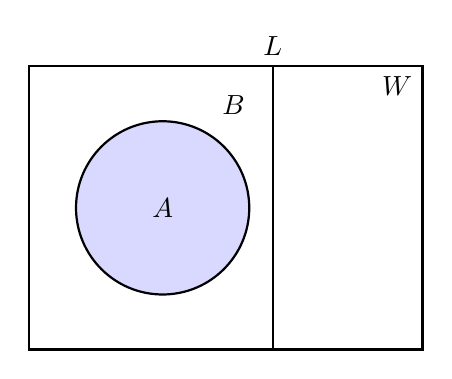
\begin{tikzpicture}[scale=1.0]
  \draw[thick] (-2.5, -1.8) rectangle (2.5, 1.8) node[below left] {$W$};
  \draw[thick, fill=blue!15] (-0.8, 0) circle (1.1) node {$A$};
  \draw[thick] (0.6, -1.8) -- (0.6, 1.8) node[above] {$L$};
  \node at (0.1, 1.3) {$B$};
\end{tikzpicture}
\caption{基集 $W$ 中的圓形點集 $A$ 與半平面點集 $B$ 補集示意}\label{fig:ground_set_complement}
\end{figure}

則 $\sim A$ 是圓外的點所成的集合，$\sim B$ 是直線右邊及直線上的點所成的集合。

請同學們自行找出 $\sim(A \cup B)$，$\sim(A \cap B)$，$(\sim A) \cap B$，$A \cap (\sim B)$，$(\sim A) \cup B$，$A \cup (\sim B)$，$(\sim A) \cap (\sim B)$，$(\sim A) \cup (\sim B)$，$\sim(A \cap (\sim B))$，$\sim(A \cup (\sim B))$ 等集合所表的區域，看看哪些是相同的集合。
\end{example}

假如 $A$ 是由性質 $\alpha$ 所定（亦即由性質 $\alpha$ 所描述），$B$ 是由性質 $\beta$ 所定，則：
\begin{itemize}
  \item $\sim A$ 是由那些不具有性質 $\alpha$ 的元素所成的集合；
  \item $\sim B$ 是由那些不具有性質 $\beta$ 的元素所成的集合。
\end{itemize}
我們將用符號「$\sim \alpha$」表示「$\alpha$ 的否定」（亦即不具有 $\alpha$）。

要注意：$\alpha$ 之否定，只有在基集 $W$ 確定時，才有意義。設 $\alpha$ 表示「是某校高一的男生」，假定基集 $W$ 為某校高一的所有學生的集合，那麼，$\sim \alpha$ 就表示「是高一的女生」。但是假如基集 $W$ 改為該校全體學生的集合，則 $\sim \alpha$ 便不止表示高一的女生，而其他各年級的男女生也都通通包含在內。

由集合運算法則：
\begin{align*}
  \sim(A \cap B) &= W \setminus (A \cap B) = (W \setminus A) \cup (W \setminus B) = (\sim A) \cup (\sim B), \\
  \sim(A \cup B) &= W \setminus (A \cup B) = (W \setminus A) \cap (W \setminus B) = (\sim A) \cap (\sim B)。
\end{align*}

\begin{example}\label{ex:2-4-8}
設 $W$ 為某校高中全體的學生的集合，$A$ 為該校高一的學生的集合，$B$ 為該校男生的集合。那麼，$A \cap B$ 為高一男生的集合，$\sim(A \cap B)$ 為所有「非」高一男生的集合，也就是該校女生的集合與高二、高三學生集合的聯集。同學們請對 $\sim(A \cap B) = (\sim A) \cup (\sim B)$ 作類似的解釋。
\end{example}

所以從上述對應可以看出：
\begin{enumerate}[(1)]
  \item $\sim(A \cap B) = (\sim A) \cup (\sim B) \iff \sim(\alpha \text{ 和 } \beta) \iff (\sim \alpha) \text{ 或 } (\sim \beta)$。\\
  亦即語句「$\alpha$ 和 $\beta$」的否定是「$(\sim \alpha)$ 或 $(\sim \beta)$」。
  \item $\sim(A \cup B) = (\sim A) \cap (\sim B) \iff \sim(\alpha \text{ 或 } \beta) \iff (\sim \alpha) \text{ 和 } (\sim \beta)$。\\
  亦即語句「$\alpha$ 或 $\beta$」的否定是「$(\sim \alpha)$ 和 $(\sim \beta)$」。
  \item 由 $\sim(\sim A) = A$，即得
  \begin{equation}\label{eq:double_negation}
    \sim(\sim \alpha) \iff \alpha
  \end{equation}
  （亦即否定的否定就是肯定）。
\end{enumerate}

為便於同學以後查考，將集合與性質（邏輯）之間的關係，列表如下：

\begin{table}[htbp]
\centering
\small
\renewcommand{\arraystretch}{1.3}
\begin{tabular}{|c|c|}
\hline
\textbf{集合語言} & \textbf{性質（邏輯）語言} \\ \hline
$A$ & $\alpha$ \\ \hline
$B$ & $\beta$ \\ \hline
$\sim A$ & $\sim \alpha$ \\ \hline
$\sim B$ & $\sim \beta$ \\ \hline
$A \cap B$ & $\alpha$ 和 $\beta$ \\ \hline
$A \cup B$ & $\alpha$ 或 $\beta$ \\ \hline
$A \subseteq B$ & $\alpha \implies \beta$ \\ \hline
$A = B$ & $\alpha \iff \beta$ \\ \hline
\end{tabular}
\caption{集合運算與邏輯語句對應表}\label{tab:set_logic_correspondence}
\end{table}

由此對應表，我們得到極重要之結論：
\begin{center}
  \textbf{「$A \subseteq B$」和「$\sim B \subseteq \sim A$」同義。} \\[0.3em]
  \textbf{「$\alpha \implies \beta$」和「$\sim \beta \implies \sim \alpha$」同義。}
\end{center}

\begin{example}\label{ex:2-4-9}
「等邊三角形一定是等腰三角形」與「不是等腰三角形一定不是等邊三角形」同義。

「$5$ 是比 $9$ 小的整數」但「比 $9$ 小的整數不一定是 $5$」。
\end{example}

\subsection*{習題 2-5}\label{sec:ex2-5}
\addcontentsline{toc}{subsection}{習題 2-5}

\begin{enumerate}[1., leftmargin=2em]
  \item 找出下列各補集來：
  \begin{enumerate}[(i)]
    \item $A$ 為正整數的集合，基集為所有整數的集合，$\sim A$ 是什麼？
    \item $A$ 為等腰三角形所成的集合，基集為所有三角形的集合，$\sim A$ 是什麼？
    \item $A$ 為正整數的集合，$B$ 為小於 $3$ 之整數的集合，基集為整數的集合，$\sim(A \cup B)$ 是什麼？$\sim(A \cap B)$ 是什麼？
    \item $A, B$ 與 (iii) 相同，基集為所有實數的集合，$\sim(A \cup B)$ 是什麼？
  \end{enumerate}
  \item 取實數的集合 $\mathbb{R}$ 為基集，並設 $A$ 為正數的集合，$B$ 為負數的集合，說明下列各集合：
  \begin{equation*}
    A \cap B, \quad (\sim A) \cap (\sim B), \quad (\sim A) \cup (\sim B), \quad (\sim A) \cup B, \quad A \cup (\sim B)。
  \end{equation*}
  \item 取 $W$ 為基集，試證：
  \begin{enumerate}[(i)]
    \item $\sim W = \emptyset$。
    \item $\sim \emptyset = W$。
    \item $A \cup (\sim A) = W$。
    \item $A \cap (\sim A) = \emptyset$。
  \end{enumerate}
  \item[*] 取自然數的集合 $\mathbb{N}$ 為基集，設 $\alpha$ 表示「是 $a$ 的倍數」的性質，$\beta$ 表示「是 $b$ 的倍數」的性質，假定 $\alpha \longleftrightarrow A$，$\beta \longleftrightarrow B$，請證明：
  \begin{enumerate}[(i)]
    \item $A \subseteq B \iff a \text{ 是 } b \text{ 的倍數}$。
    \item $A \cap B = \{x \mid x \text{ 是 } a, b \text{ 最小公倍數的倍數}\}$。
  \end{enumerate}
  \item 假定：(i)「$\alpha$ 或 $\beta \implies \gamma$」及 (ii)「$\alpha$ 或 $\sim \beta \implies \gamma$」均成立，試證「$\alpha \implies \gamma$」亦成立。（參照習題 2-3，第 10 題）
\end{enumerate}

\subsection*{附錄：羅馬數字乘法運算}\label{sec:ch2-appendix}
\addcontentsline{toc}{subsection}{附錄：羅馬數字乘法運算}

像 $365 \times 24 = 8760$ 這個乘式運算，若以羅馬數字符號表示，就成為以下複雜繁瑣的樣子：
\begin{align*}
  & (\mathrm{CCCLXV}) \cdot (\mathrm{XXIV}) \\
  &= (\mathrm{C}+\mathrm{C}+\mathrm{C}+\mathrm{L}+\mathrm{X}+\mathrm{V}) \cdot (\mathrm{X}+\mathrm{X}+\mathrm{V}-\mathrm{I}) \\
  &= \mathrm{C}\cdot\mathrm{X} + \mathrm{C}\cdot\mathrm{X} + \mathrm{C}\cdot\mathrm{X} + \mathrm{L}\cdot\mathrm{X} + \mathrm{X}\cdot\mathrm{X} + \mathrm{V}\cdot\mathrm{X} \\
  &\quad + \mathrm{C}\cdot\mathrm{X} + \mathrm{C}\cdot\mathrm{X} + \mathrm{C}\cdot\mathrm{X} + \mathrm{L}\cdot\mathrm{X} + \mathrm{X}\cdot\mathrm{X} + \mathrm{V}\cdot\mathrm{X} \\
  &\quad + \mathrm{C}\cdot\mathrm{V} + \mathrm{C}\cdot\mathrm{V} + \mathrm{C}\cdot\mathrm{V} + \mathrm{L}\cdot\mathrm{V} + \mathrm{X}\cdot\mathrm{V} + \mathrm{V}\cdot\mathrm{V} \\
  &\quad - \mathrm{C} - \mathrm{C} - \mathrm{C} - \mathrm{L} - \mathrm{X} - \mathrm{V} \\
  &= \mathrm{M}+\mathrm{M}+\mathrm{M}+\mathrm{D}+\mathrm{C}+\mathrm{L} + \mathrm{M}+\mathrm{M}+\mathrm{M}+\mathrm{D}+\mathrm{C}+\mathrm{L} \\
  &\quad + \mathrm{D}+\mathrm{D}+\mathrm{D}+\mathrm{C}+\mathrm{C}+\mathrm{L}+\mathrm{L}+\mathrm{X}+\mathrm{X}+\mathrm{V} - \mathrm{C} - \mathrm{C} - \mathrm{C} - \mathrm{L} - \mathrm{X} - \mathrm{V} \\
  &= \mathrm{M}+\mathrm{M}+\mathrm{M}+\mathrm{M}+\mathrm{M}+\mathrm{M}+\mathrm{M}+\mathrm{C}+\mathrm{C}+\mathrm{C}+\mathrm{M}+\mathrm{D}+\mathrm{C}+\mathrm{C}+\mathrm{C}+\mathrm{X}+\mathrm{X}+\mathrm{V} \\
  &\quad - \mathrm{C} - \mathrm{C} - \mathrm{C} - \mathrm{L} + \mathrm{X} - \mathrm{V} \\
  &= \mathrm{M}+\mathrm{M}+\mathrm{M}+\mathrm{M}+\mathrm{M}+\mathrm{M}+\mathrm{M}+\mathrm{M}+\mathrm{D}+\mathrm{C}+\mathrm{C}+\mathrm{C} - \mathrm{L} + \mathrm{X} \\
  &= \mathrm{M}+\mathrm{M}+\mathrm{M}+\mathrm{M}+\mathrm{M}+\mathrm{M}+\mathrm{M}+\mathrm{M}+\mathrm{D}+\mathrm{C}+\mathrm{C}+\mathrm{L}+\mathrm{X} \\
  &= \mathrm{MMMMMMMMDCCLX} \quad (= 8760)。
\end{align*}


\end{document}
